\documentclass[xcolor=dvipsnames]{beamer}
\usepackage[T1]{fontenc}
\usepackage[utf8]{inputenc}
\usepackage[english,slovak]{babel}

\usepackage{amsmath}
\usepackage{amsthm}
\usetheme{Pittsburgh}
\useoutertheme{shadow}

\usepackage{graphicx}
\usepackage{caption}
\usepackage{subcaption}

\usepackage[]{algorithm2e}
\usepackage{listings}
 \setbeamercovered{transparent}
 \usepackage{cuted}
\usepackage[export]{adjustbox}
\usepackage{mathtools}

\usepackage{lipsum}

\newcommand\Wider[2][3em]{%
\makebox[\linewidth][c]{%
  \begin{minipage}{\dimexpr\textwidth+#1\relax}
  \raggedright#2
  \end{minipage}%
  }%
}

%-------------------------------------------------------------------------------------
\title{\bf Deep reinforcement learning}
\author{Michal CHOVANEC, PhD.}


%\setbeamertemplate{footline}[frame number]{}
\setbeamertemplate{navigation symbols}{}


\date[EURP]{\it April 2018}
\begin{document}

\begin{frame}
\titlepage
\centering{Faculty of Management Science and Informatics}
\end{frame}


\begin{frame}{\bf Problem definition}
\begin{itemize}
 \item learn to play game with unknow rules
 \item input  : state and reward
 \item output : action and total score
 \item $Q(s, a)$ : learn Q function
\end{itemize}
\centering

{\color{red} \bf agent never sees required value (required action)}


\begin{figure}
\centering
\begin{minipage}{.5\textwidth}
  \centering
  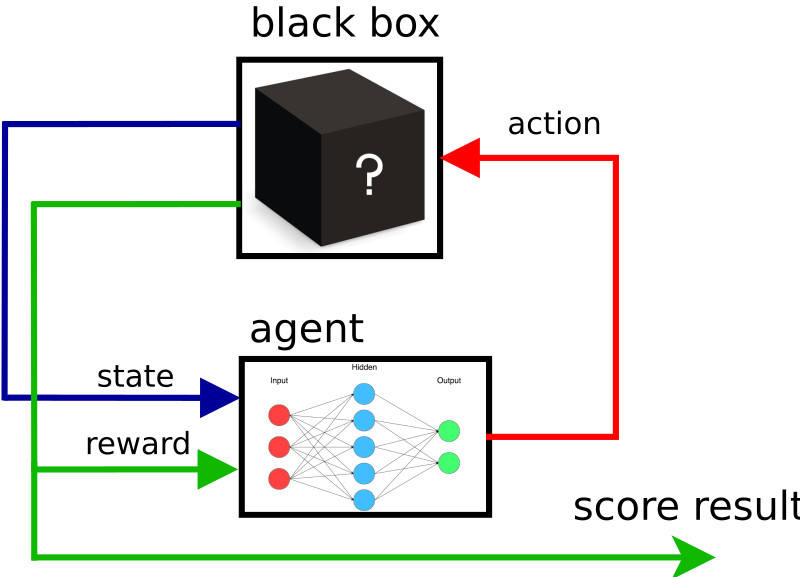
\includegraphics[scale=0.2]{../../diagrams/rl_mechanism.jpg}
\end{minipage}%
\begin{minipage}{.5\textwidth}
  \centering
  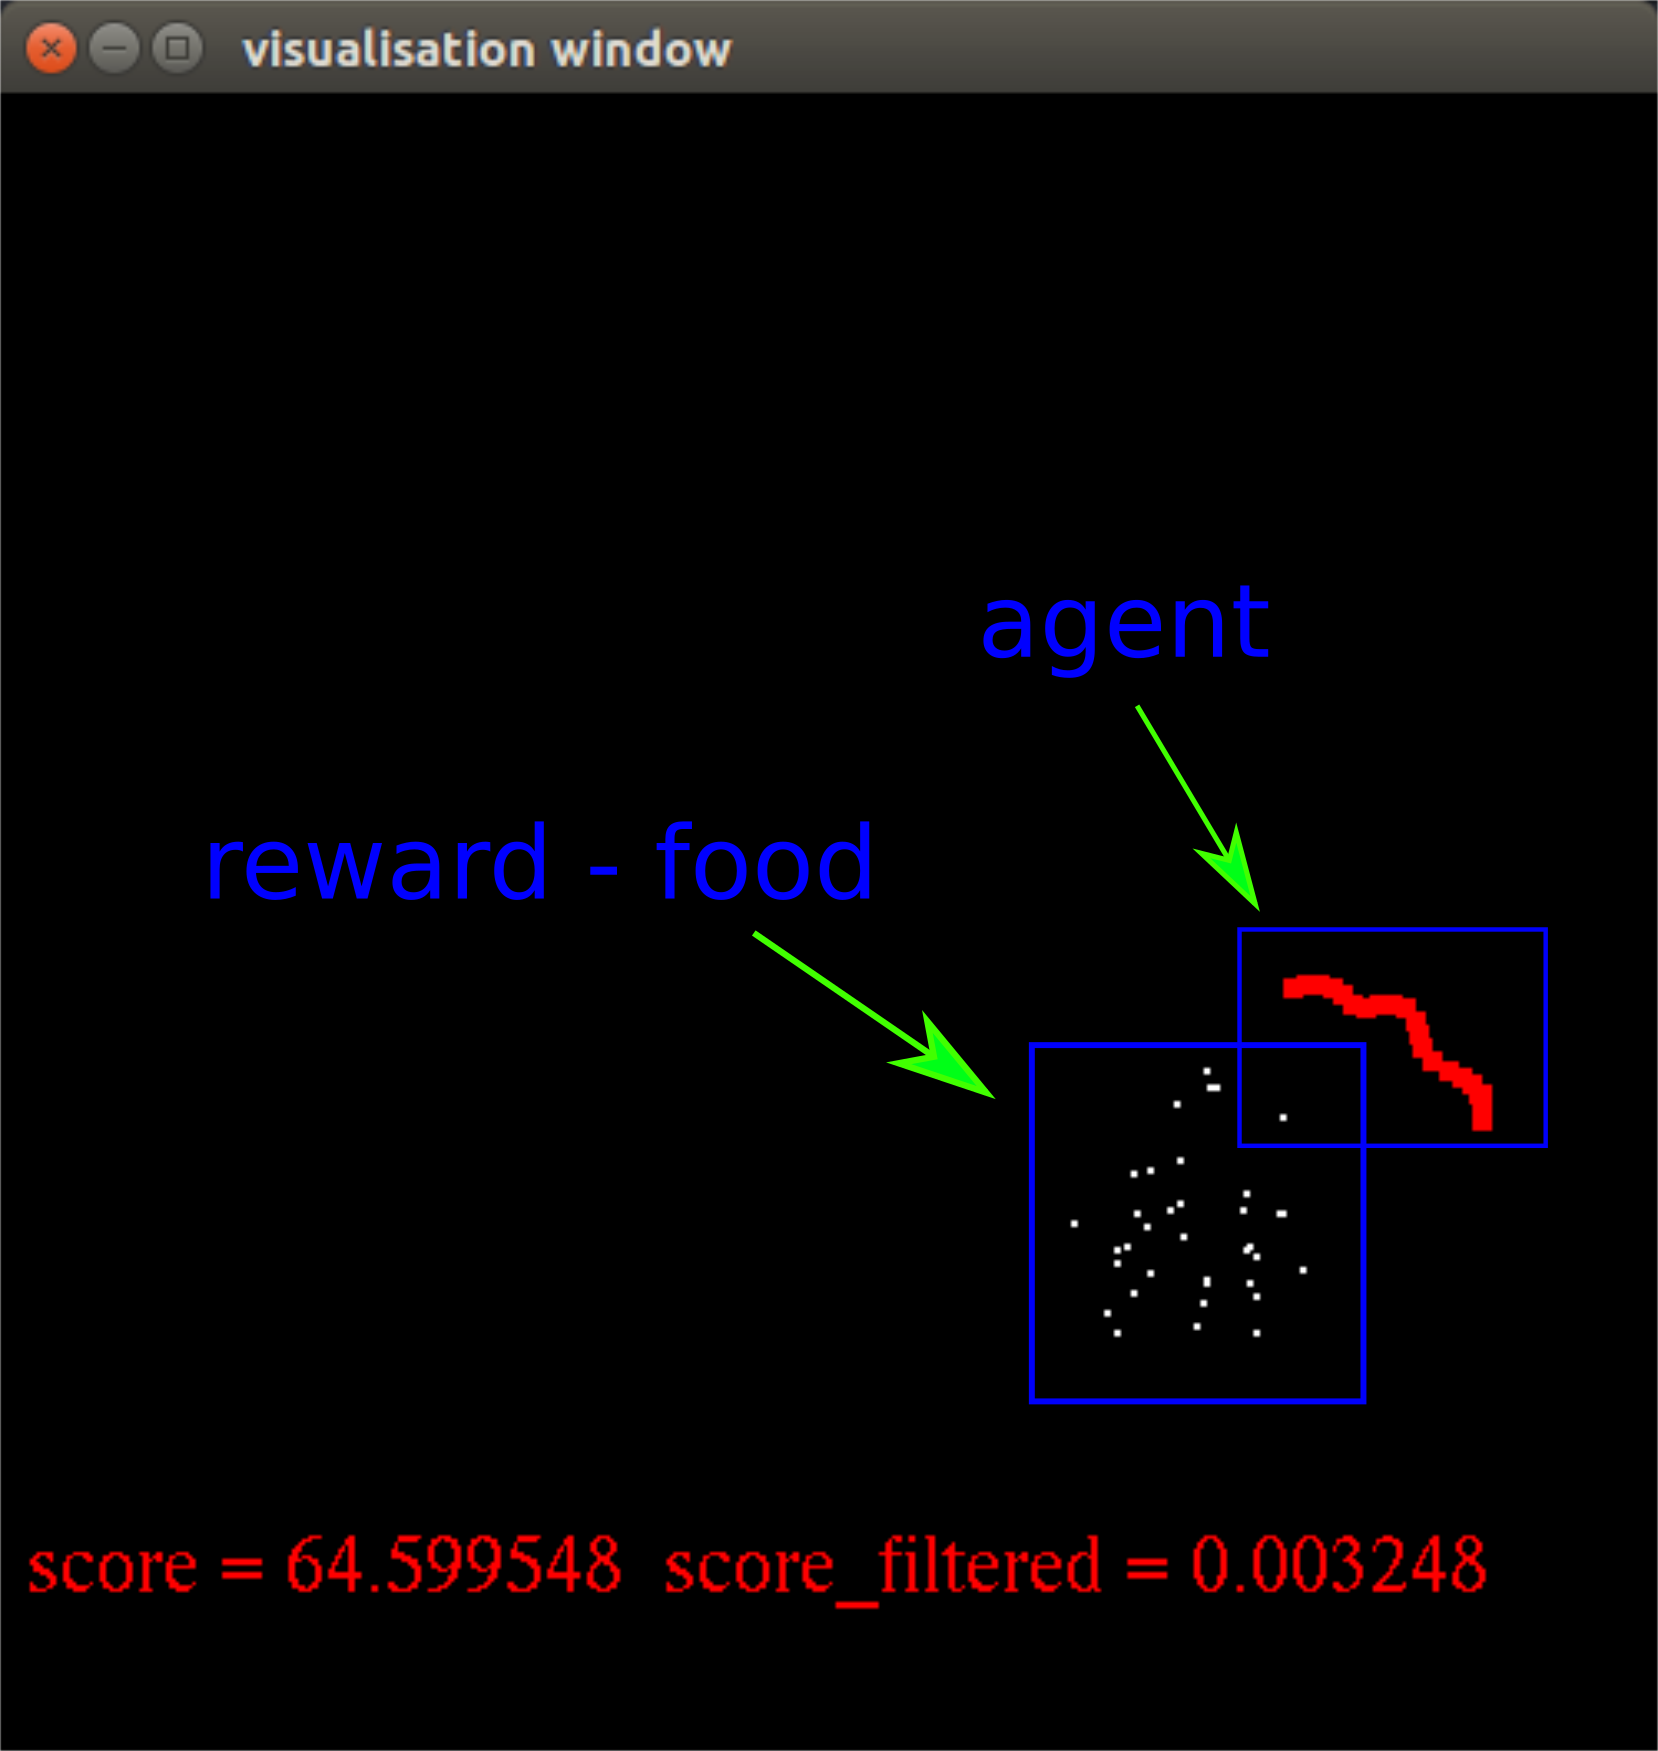
\includegraphics[scale=0.2]{../../diagrams/worms_rl_game_desc.png}
\end{minipage}
\end{figure}



\end{frame}


\begin{frame}{\bf Storing Q values}

\begin{itemize}
 \item table
 \item linear combination of basis function (handmade features)
 \item Kenerva's sparse encoding
 \item neural network
\end{itemize}

problems
\begin{itemize}
 \item state correlations
 \item nonstationary Q values
 \item convergence to optimal strategy
\end{itemize}

\end{frame}


\begin{frame}{\bf Neural network approximator - deep reinforcement learning}

\begin{figure}[htbp]
  \centering
  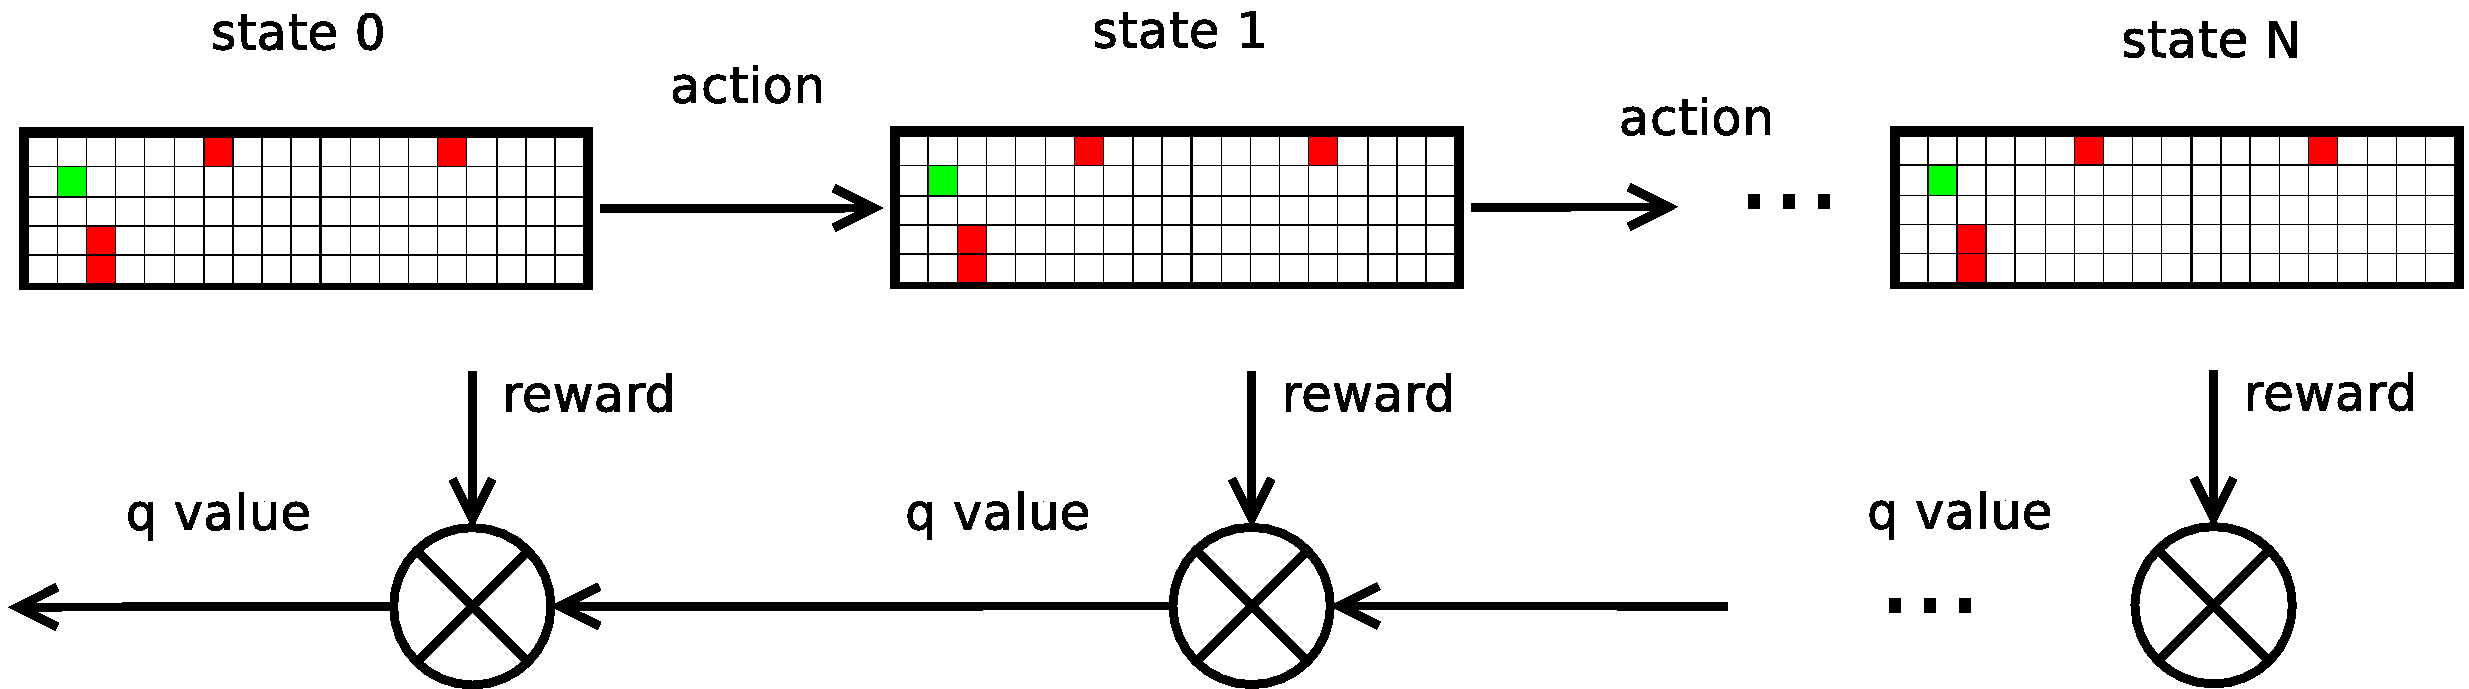
\includegraphics[scale=0.3]{../../diagrams/rl_nn_learn.png}
\end{figure}


\begin{figure}[htbp]
  \centering
  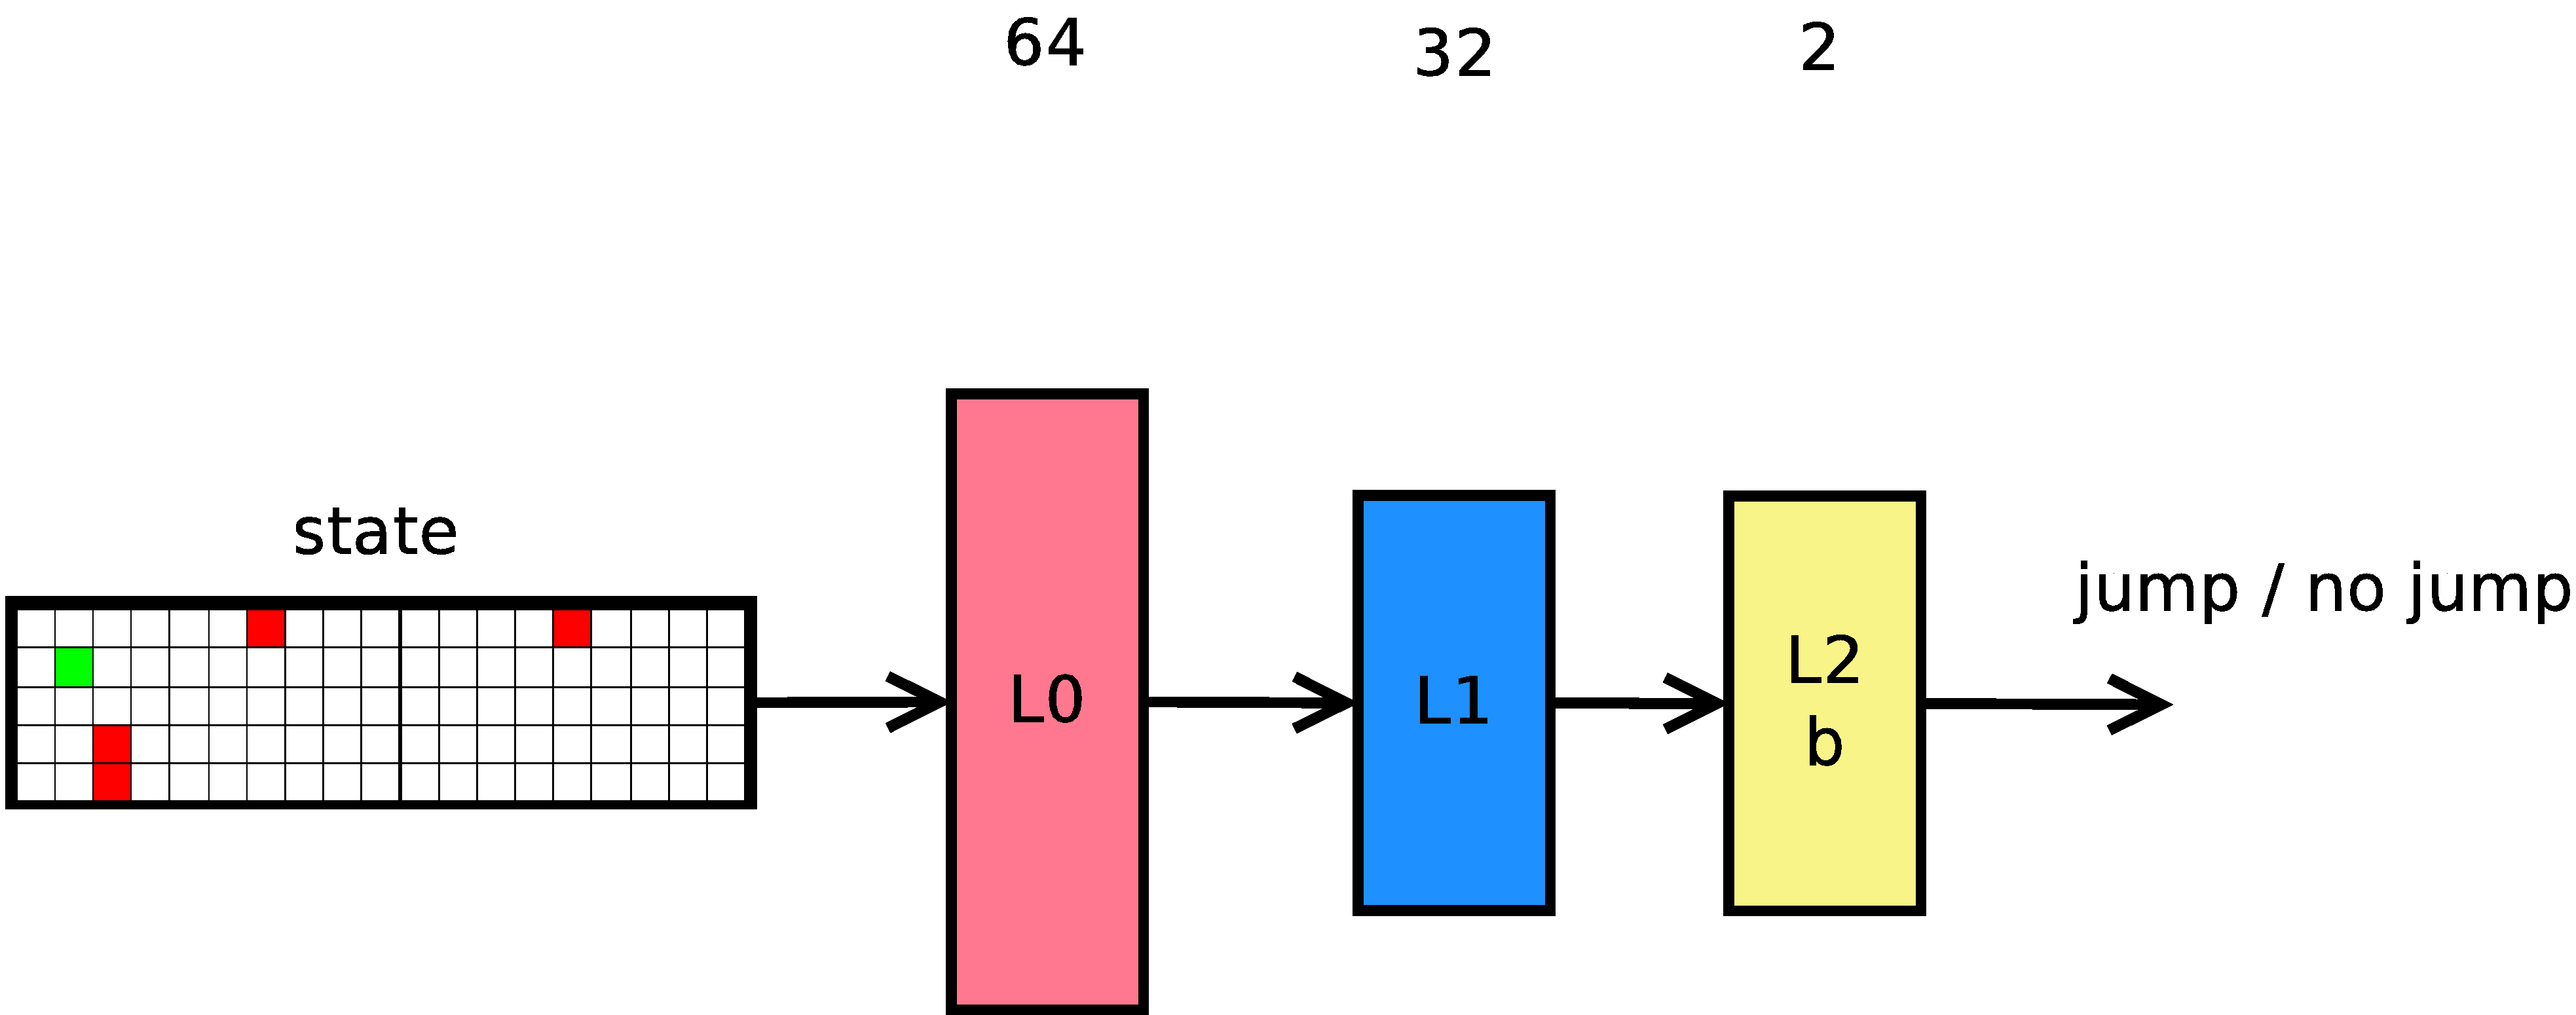
\includegraphics[scale=0.3]{../../diagrams/fnn.png}
\end{figure}

\end{frame}



\begin{frame}{\bf Speed up learning}

\begin{figure}[htbp]
  \centering
  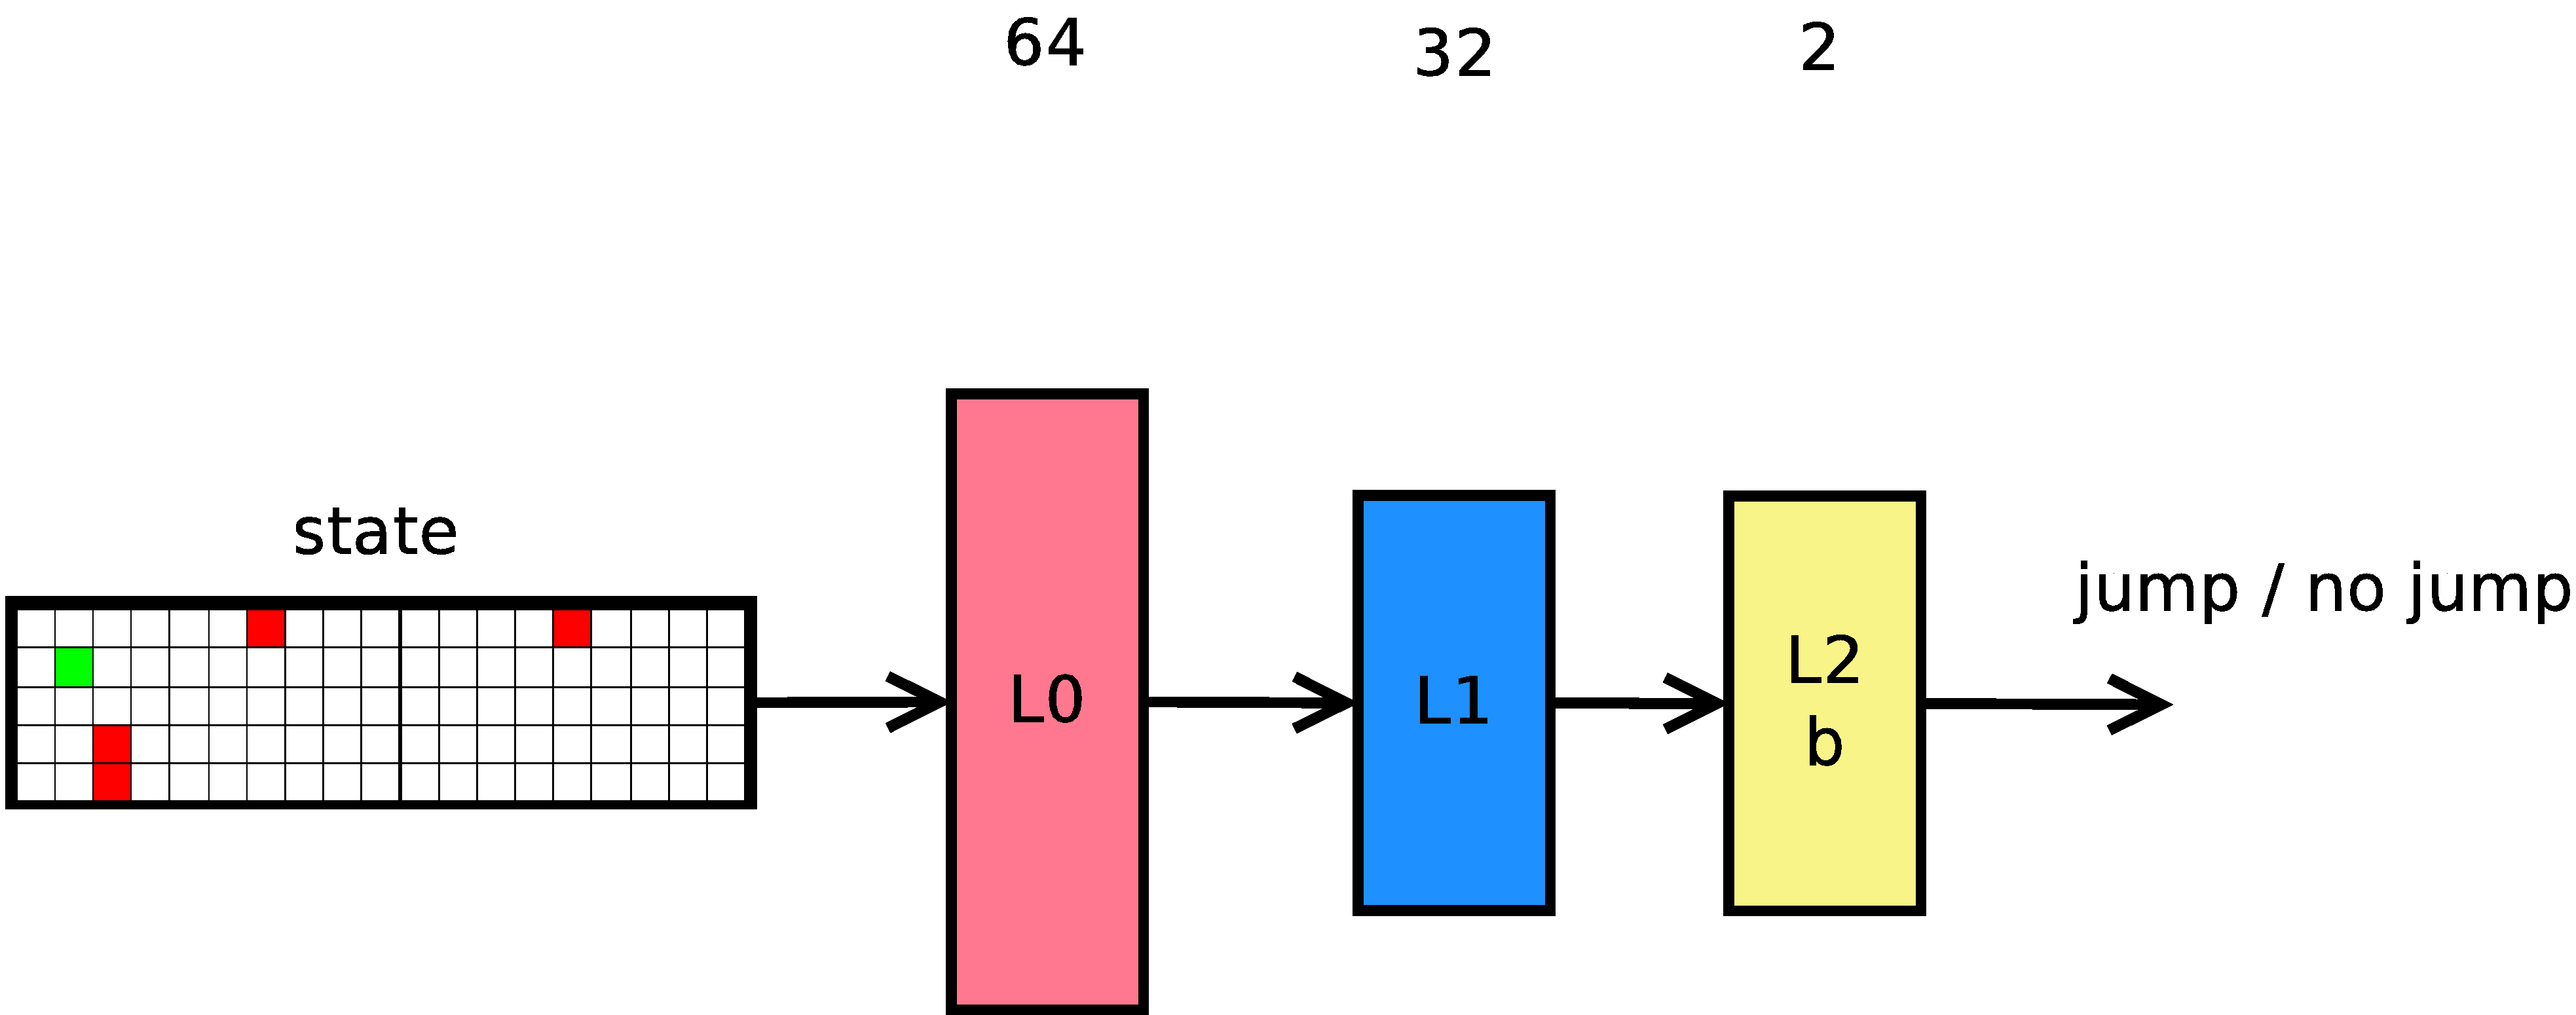
\includegraphics[scale=0.21]{../../diagrams/fnn.png}
  \caption*{common feed forward neural network}
\end{figure}

\begin{figure}[htbp]
  \centering
  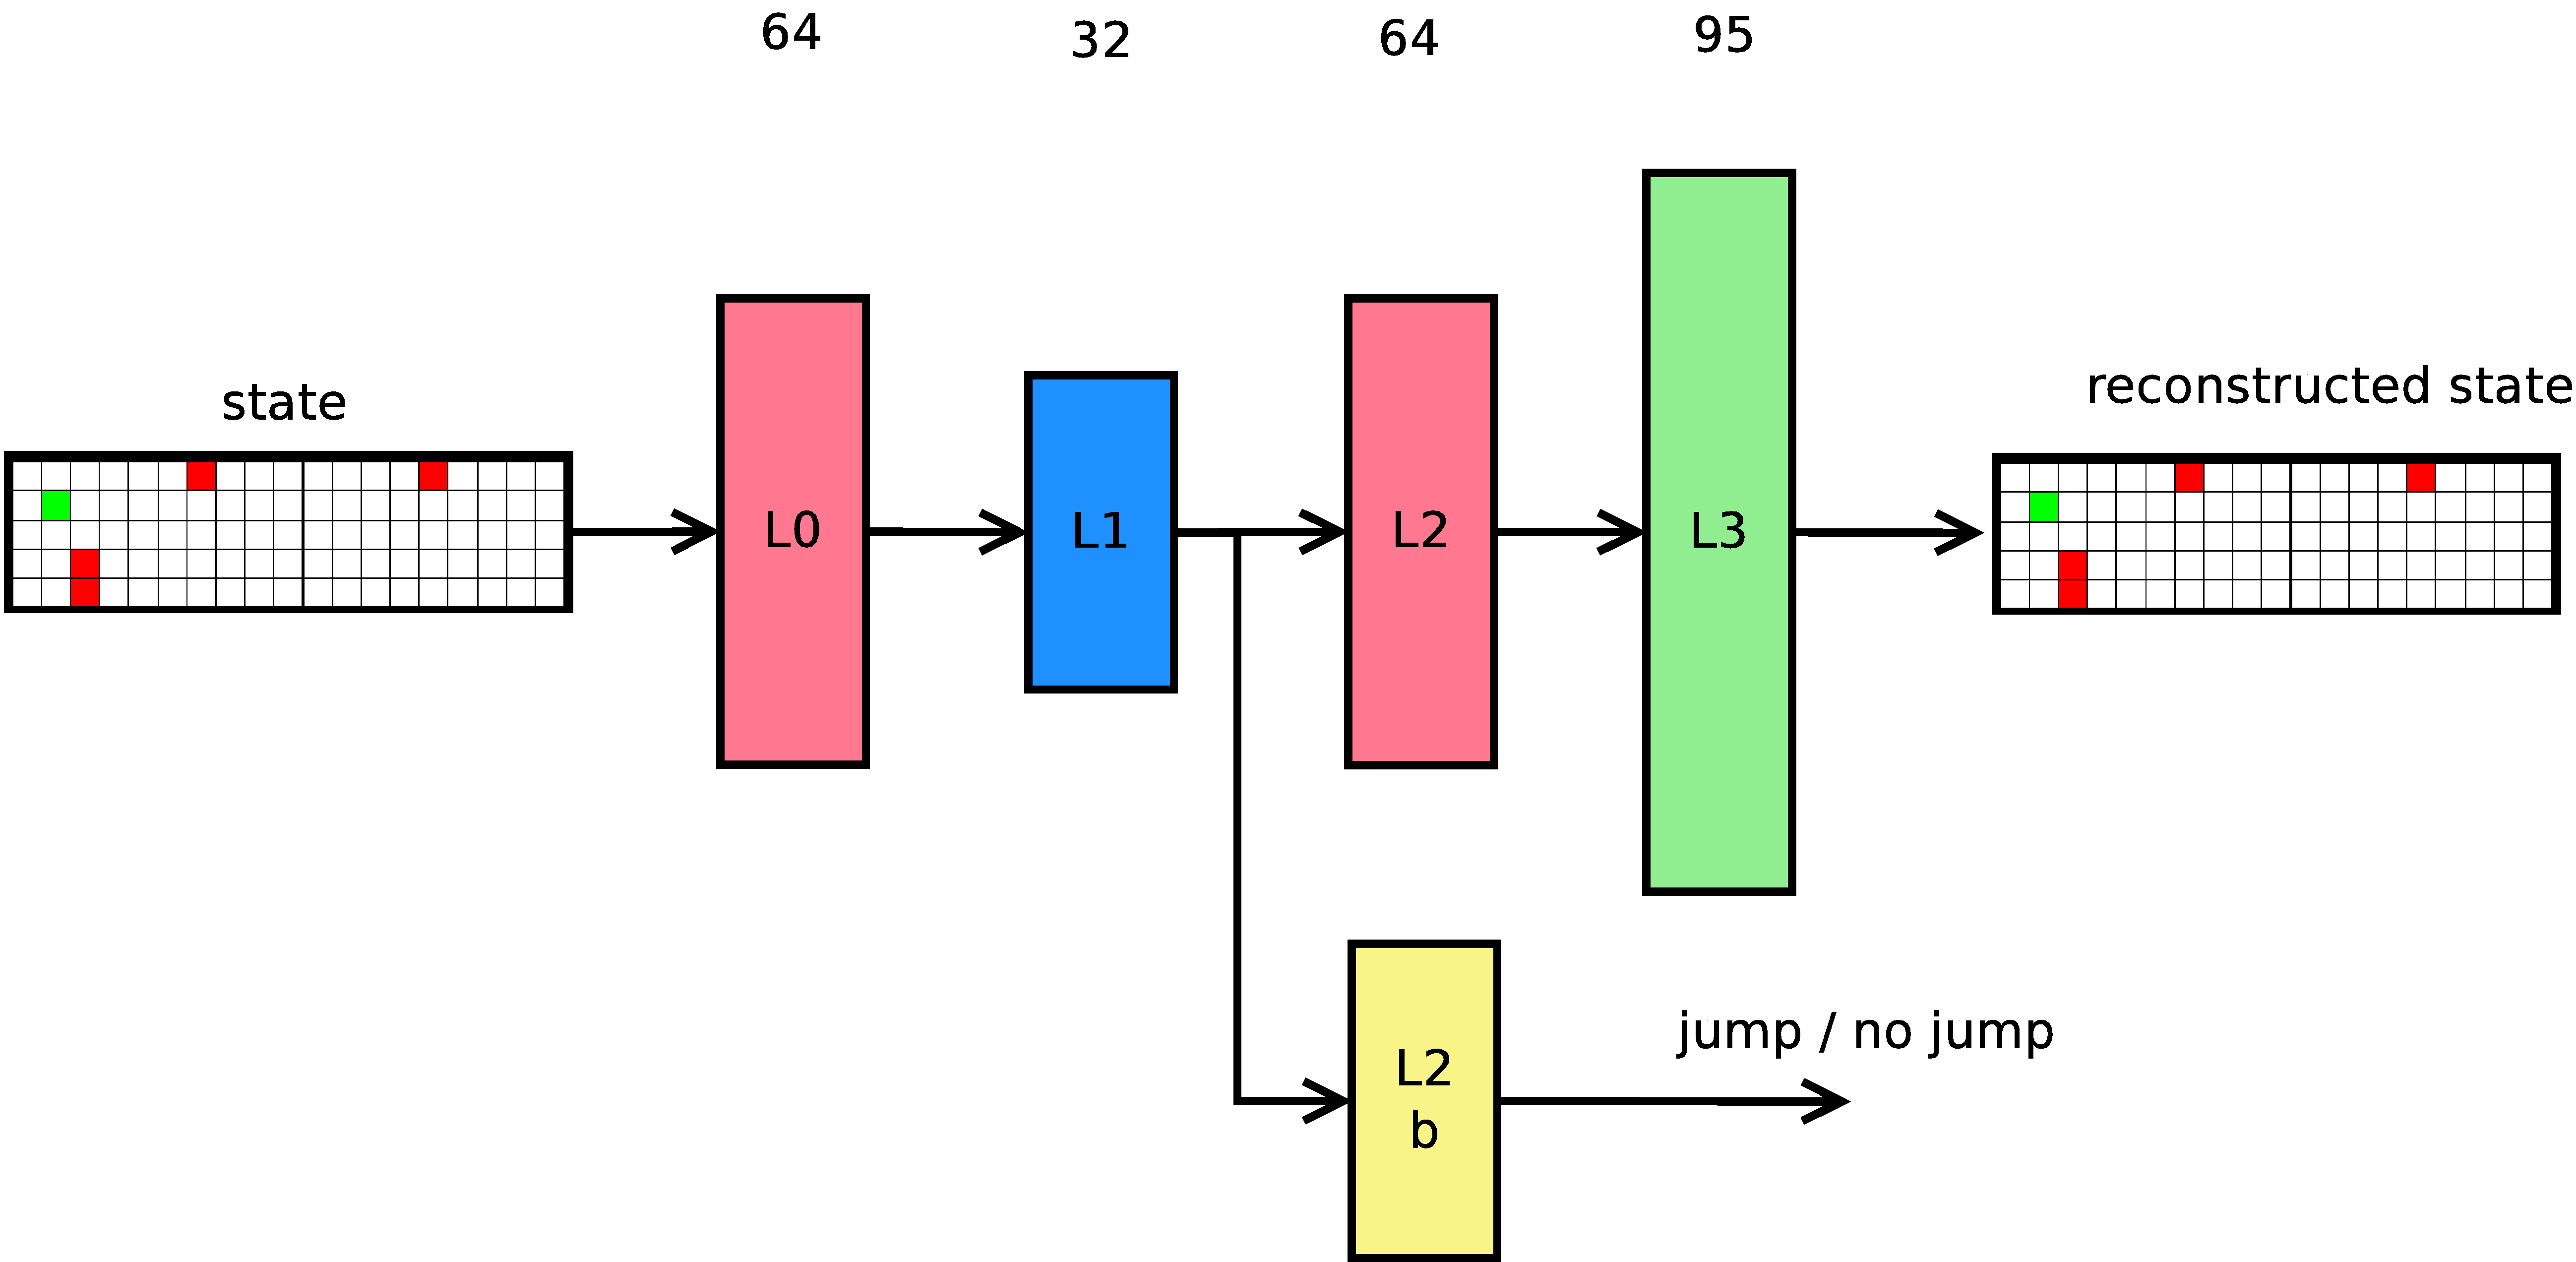
\includegraphics[scale=0.21]{../../diagrams/hnn.png}
  \caption*{stacked autoencoder + feed forward neural network}
\end{figure}

\end{frame}

\begin{frame}{\bf Arcade game experiment}


\begin{figure}[htbp]
  \centering
  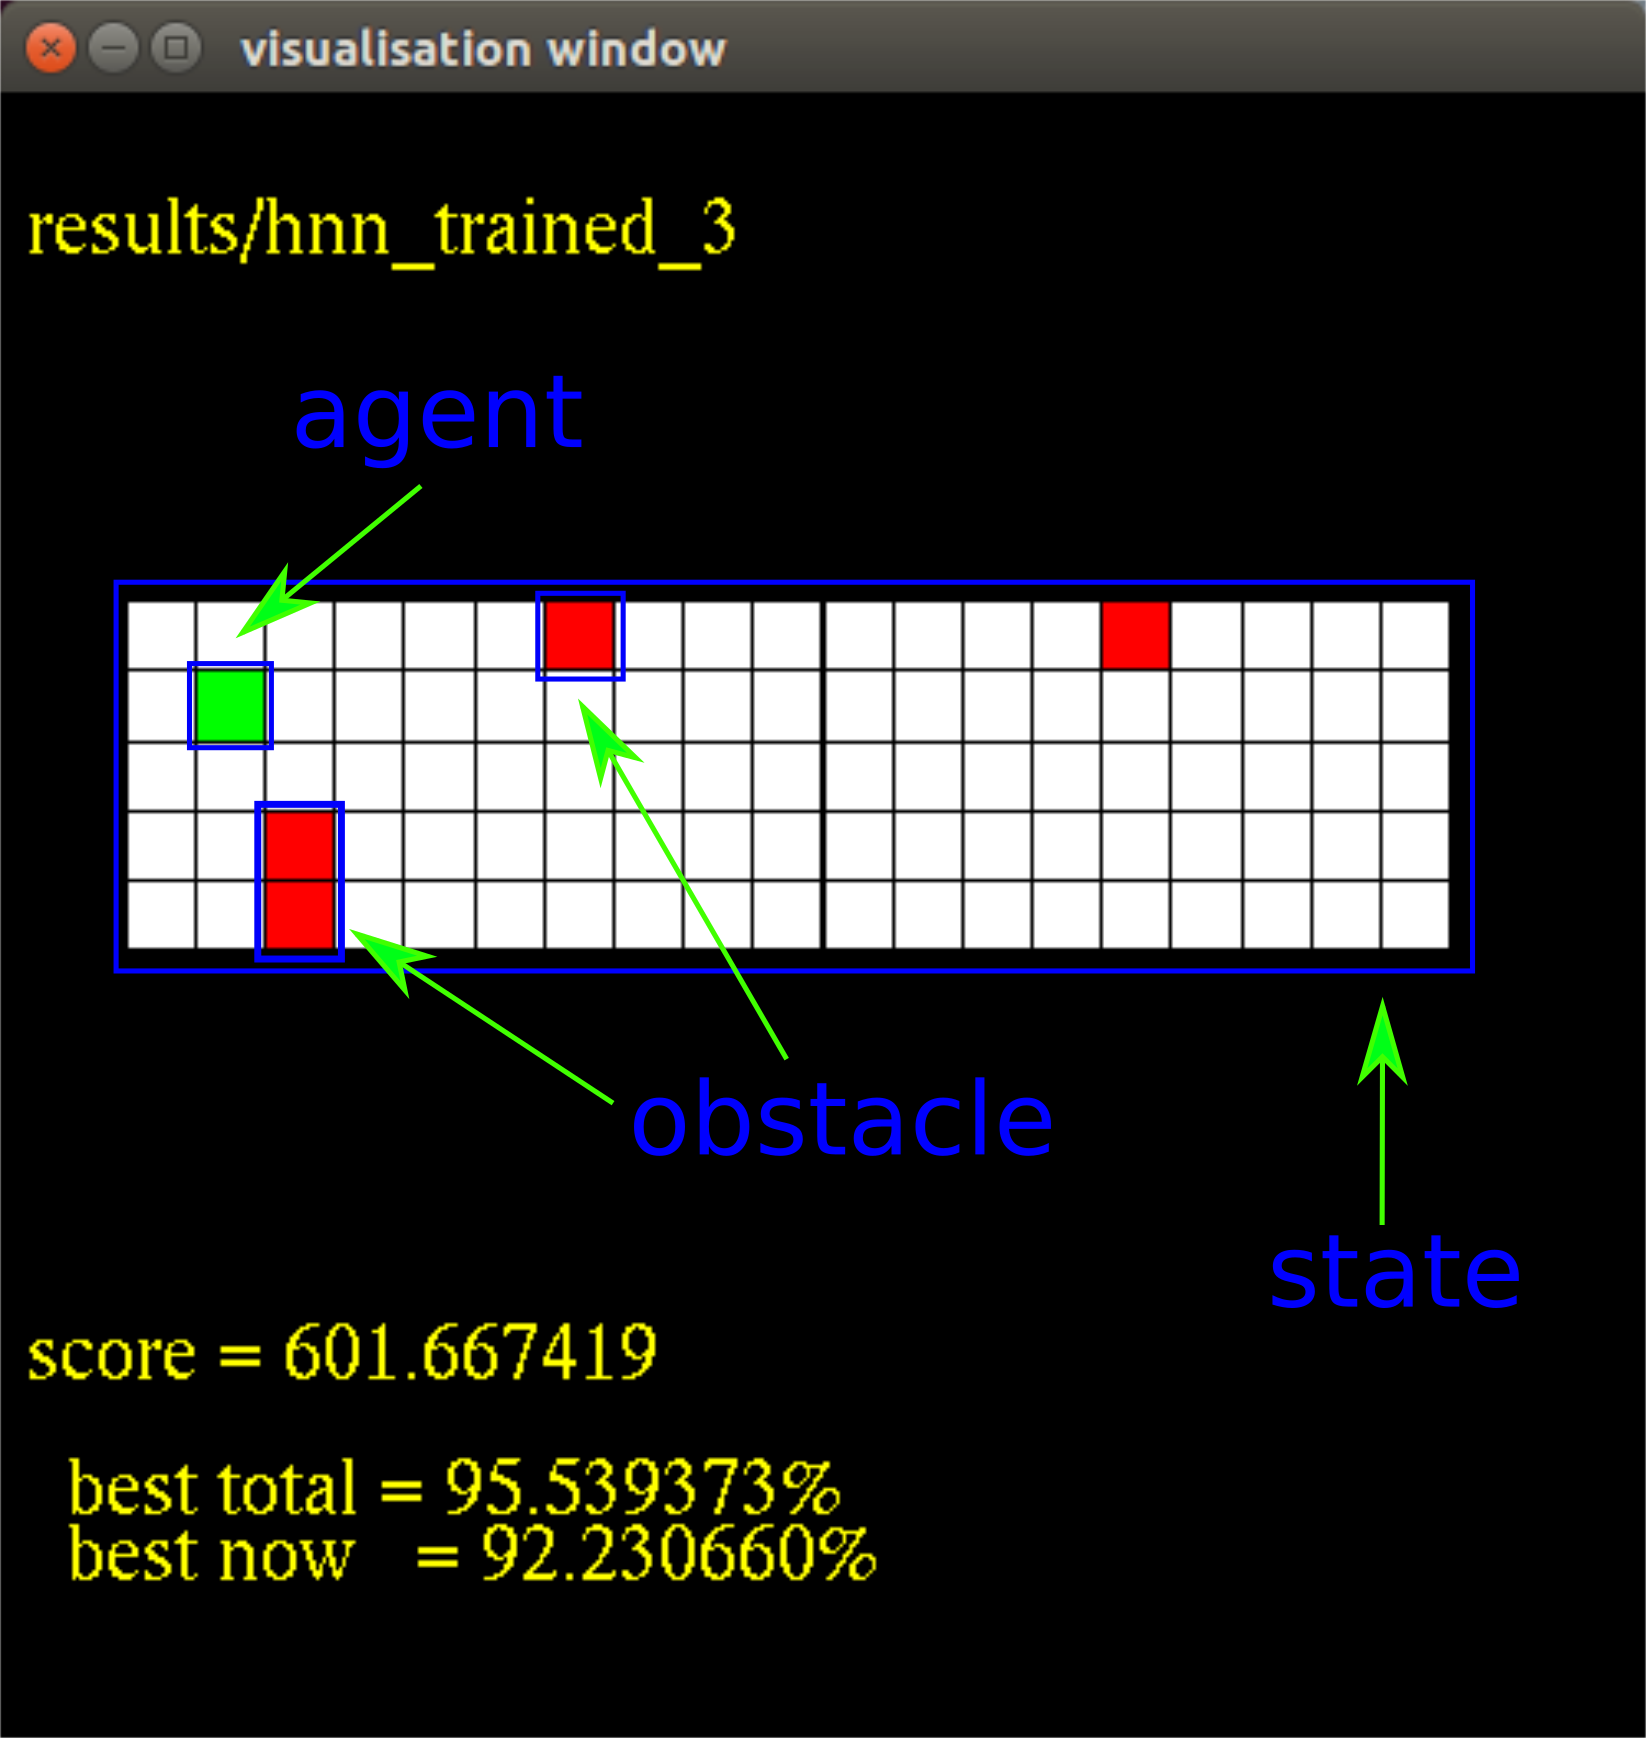
\includegraphics[scale=0.21]{../../diagrams/arcade_rl_game_desc.png}
\end{figure}

{
\tiny

\begin{table}[!h]
\centering
\begin{tabular}{|l|l|l|l|l|}
\hline
                        & FNN sparse & FNN no sparse & AE+FNN  sparse & AE+FNN no sparse \\ \hline
unsupervised iterations & 0          & 0             & 100000         & 100000           \\ \hline
supervised iterations   & 200000     & 200000        & 200000         & 200000           \\ \hline
iterations per slice    & 0          & 0             & 50000          & 50000            \\ \hline
learning rate           & 0.0005     & 0.0005        & 0.0005         & 0.0005           \\ \hline
init weight range       & 0.1        & 0.1           & 0.1            & 0.1              \\ \hline
dropout                 & 0          & 0             & 0              & 0                \\ \hline
lambda                  & 0.00000001 & 0             & 0.00000001     & 0                \\ \hline
\end{tabular}
\end{table}

}

\end{frame}




\begin{frame}{\bf Results}


\begin{figure}[!h]
  \centering
  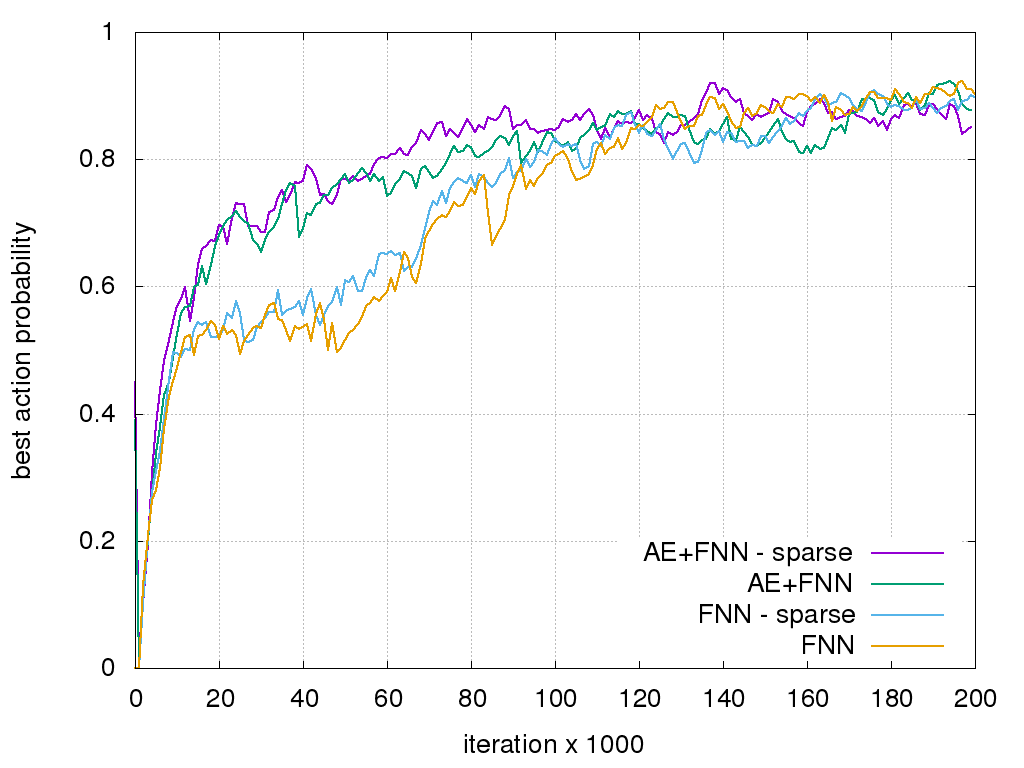
\includegraphics[scale=0.25]{../../results/rl_arcade/training_progress.png}
  \caption*{Average training progress comparison}
  \label{img:Average training progress comparison}
\end{figure}

{
\tiny
\begin{table}[]
\centering
\label{tab:summary_results}
\begin{tabular}{|l|c|c|c|c|}
\hline
                         & \multicolumn{1}{l|}{average score} & \multicolumn{1}{l|}{best score} & \multicolumn{1}{l|}{worst score} & \multicolumn{1}{l|}{average best action probability {[}\%{]}} \\ \hline
FNN sparse weights       & 957.31                             & 978.3                          & 927.31                           & 94.04                                                       \\ \hline
FNN nosparse weights     & 951.5                             & 959.3                          & 942.644                           & 95.95                                                   \\ \hline
AE+FNN sparse weights    & 763.58                             & 942.97                          & 618.66                           & 88.16                                                       \\ \hline
AE+FNN no sparse weights & 737.78                             & 884.98                          & 618.99                           & 87.19                                                        \\ \hline
\end{tabular}
\end{table}
}

\end{frame}












\begin{frame}{\bf Snake game experiment}


\begin{figure}[htbp]
  \centering
  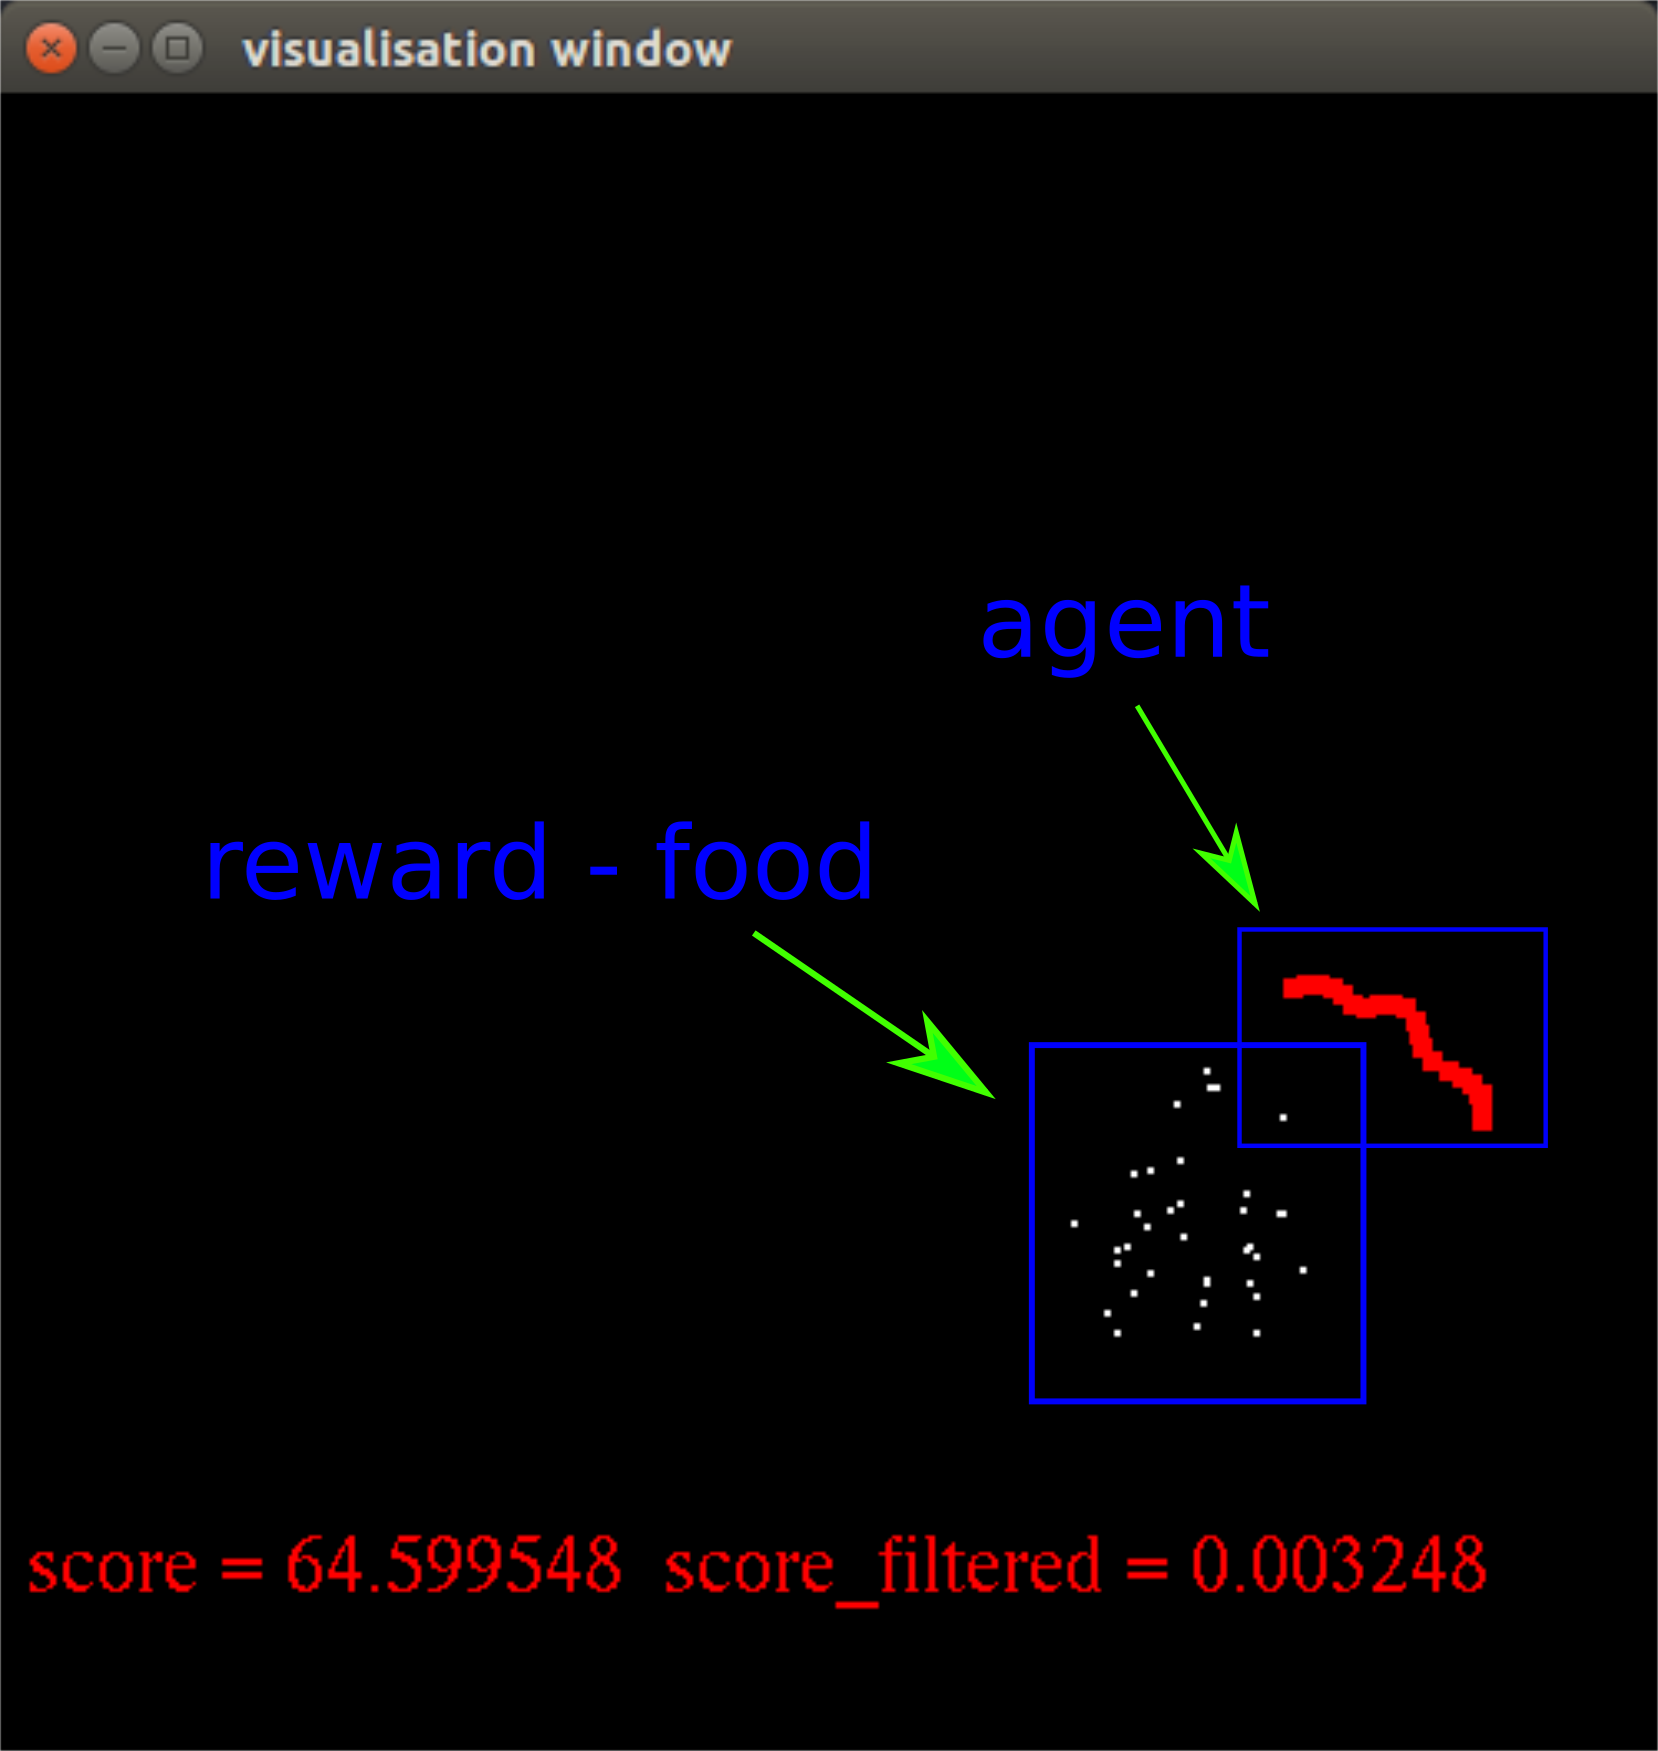
\includegraphics[scale=0.15]{../../diagrams/worms_rl_game_desc.png}
\end{figure}

\begin{figure}[!htb]
\centering
\begin{minipage}{.5\textwidth}
  \centering
  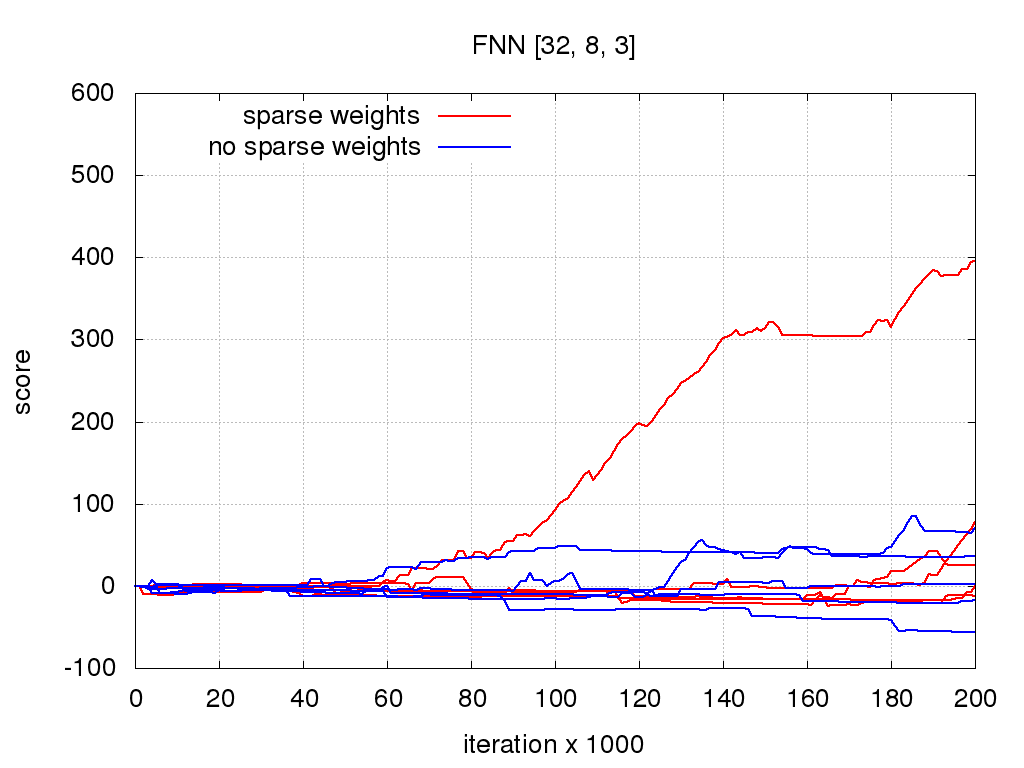
\includegraphics[scale=0.17]{../../results/rl_worms/fnn_progress/training_progress.png}
  \captionof*{figure}{FNN score progress comparison}
  \label{img:worms FNN score progress comparison}
\end{minipage}%
\begin{minipage}{.5\textwidth}
  \centering
  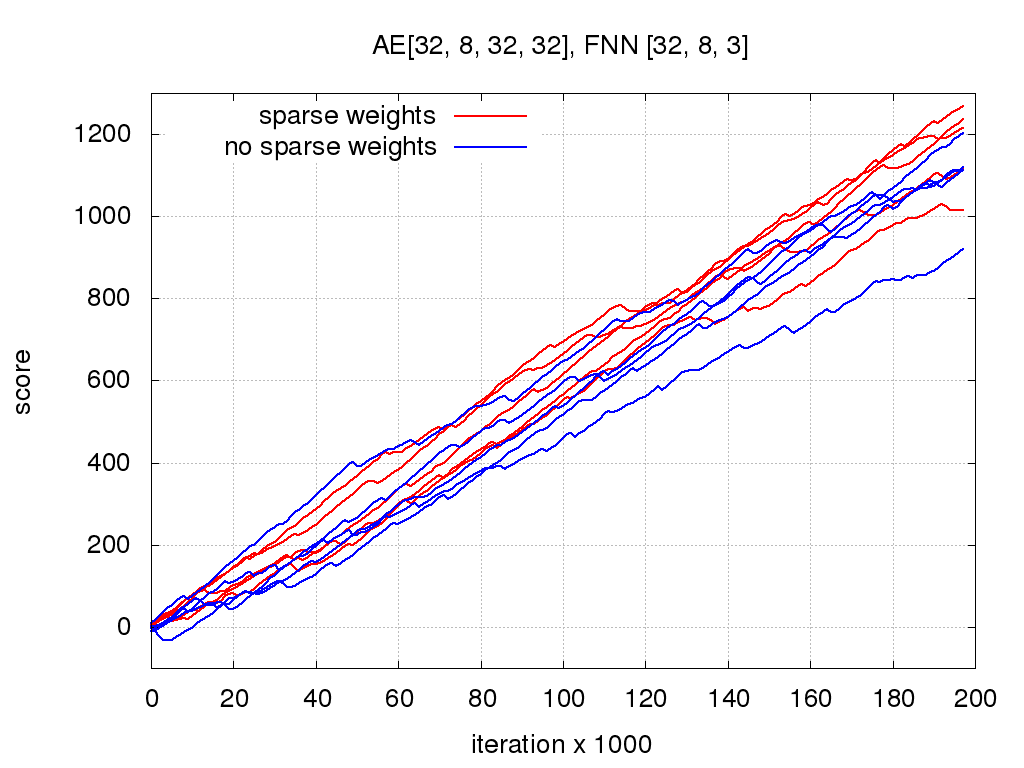
\includegraphics[scale=0.17]{../../results/rl_worms/hnn_progress/training_progress.png}
  \captionof*{figure}{AE+FNN score progress comparison}
  \label{img:worms AE+FNN score progress comparison}
\end{minipage}
\end{figure}

\end{frame}



%-------------------------------------------------------------------------------------
\begin{frame}{\bf Q\&A}

\begin{figure}[ht]
\begin{center}
\begin{minipage}{0.8\linewidth}
\begin{center}
 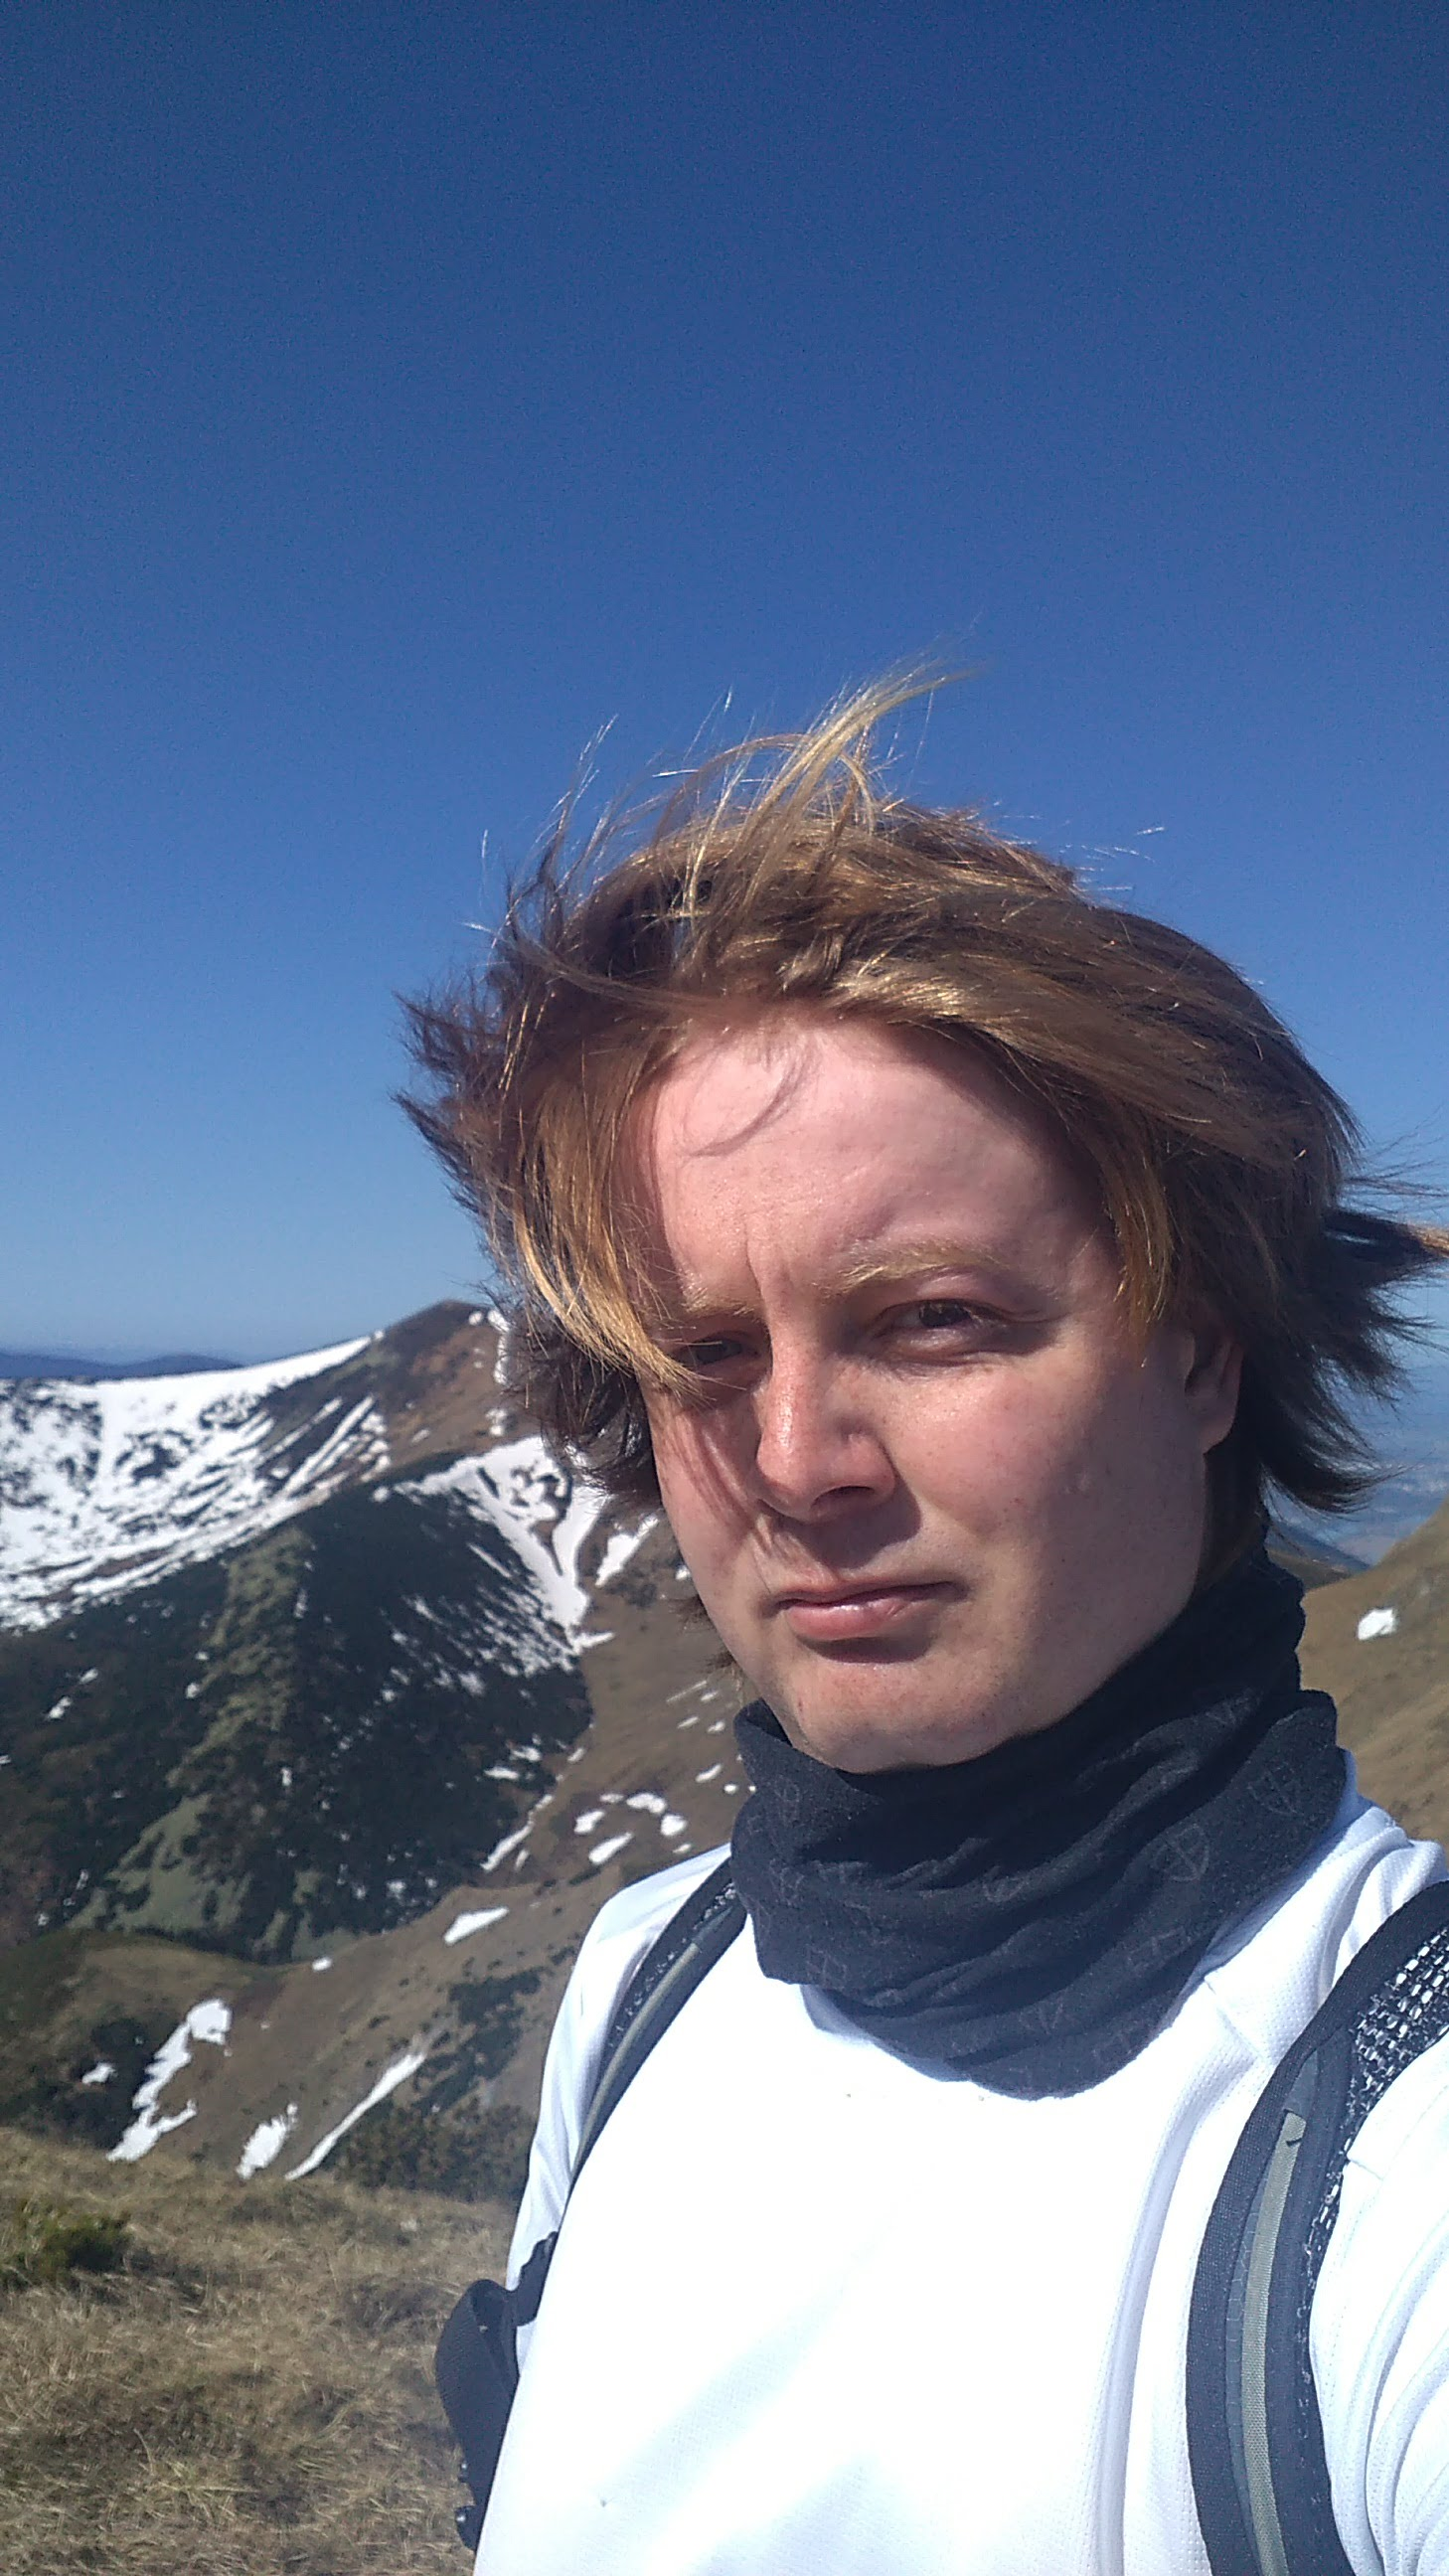
\includegraphics[width=0.35\textwidth]{../../pictures/me3.jpg}
\end{center}
\end{minipage}
\end{center}
\end{figure}

\url{https://github.com/michalnand/robotics}
\url{https://github.com/michalnand/machine\_learning}

\centerline{michal.nand@gmail.com}

\end{frame}

\end{document}
